\section[Gradiente radiativo]{Gradiente radiativo e criterio di Schwarzschild}\label{sec:gradiente-radiativo}
L'equazione del \emph{gradiente radiativo} fornisce il profilo radiale delle variazioni di $T$ all'interno della stella. Si può scrivere:
\begin{equation}\label{eq:gradiente-radiativo}
    \dfrac{\ud T}{\ud r}\Big|_\textup{rad} = - \dfrac{3 \kappa \rho}{4 \pi r^2} \dfrac{L(r)}{4 a c T^3}
\end{equation}
Essa mostra che l'opacità e il flusso radiativo determinano quanto rapidamente $T$ varia con $r$.

Utilizzando questa equazione è possibile determinare quando c'è convezione nella stella, utilizzando il seguente \emph{criterio di Schwarzscild}:
\begin{equation}\label{eq:criterio-schwarzscild}
    \text{se} \quad \abs*{\dfrac{\ud T}{\ud r}}_\textup{rad} > \abs*{\dfrac{\ud T}{\ud r}}_\textup{ad} \implies \text{c'è convezione.}
\end{equation}
in particolare, quando il criterio è verificato avverrà la convezione.

\subsection{Ricavare l'equazione}
Per trovare il gradiente radiativo prima di tutto ricaviamo il gradiente di pressione di radiazione, derivando rispetto a $r$ l'espressione~\eqref{eq:pressione-radiazione}. Si ottiene:
\[
\dfrac{\ud P_\textup{rad}}{\ud r} = \frac{4}{3} a T^3 \dfrac{\ud T}{\ud r}
\] 
d'altra parte, il gradiente di radiazione dipende anche dall'\emph{opacità} e dal \emph{flusso} di radiazione. Si ricorda che l'opacità $\kappa$ era stata introdotta nell'eq.~\eqref{eq:trasporto-radiativo} del par.~\ref{sec:soluzioni-trasporto-radiativo}, mentre il flusso, $F_\textup{rad}$, è definito dall'eq.~\eqref{eq:flusso}. In particolare, senza dare ulteriori specificazioni, possiamo esprimere il gradiente della pressione di radiazione come:
\[
\dfrac{\ud P_\textup{rad}}{\ud r} = -\dfrac{\kappa \rho}{c} F_\textup{rad}
\]
e mettendo insieme le utlime due relazioni si ottiene:
\[
\dfrac{\ud T}{\ud r}\Big|_\textup{rad} = - \dfrac{3}{4ac} \dfrac{\kappa \rho}{T^3} F_\textup{rad}
\]
con
\[
F_\textup{rad} = \dfrac{L_r}{4 \pi r^2}
\]
da cui segue immediatamente la~\eqref{eq:gradiente-radiativo}. Come già detto, l'equazione fornisce il profilo radiale delle variazioni di $T$ con $r$ e mostra come l'opacità $\kappa$ e il flusso radiativo $F_\textup{rad}$ influiscono sulla rapidità di variazione di $T$ con $r$.

Il gradiente di temperatura ha un impatto cruciale sul meccanismo preponderante di trasporto di energia all'interno della struttura stellare. Introduciamo brevemente i meccanismi di trasporto di energia.

\subsection{Meccanismi di trasporto di energia}
I tre meccanismi di trasporto in una stella sono il \emph{trasporto radiativo}, \emph{convettivo} e \emph{conduttivo}. Di seguito ne sono elencate le principali proprietà:
\begin{description}
    \item[Trasporto conduttivo:] I principali responsabili di questo meccanismo sono gli \emph{elettroni} ed è efficiente solo se il gas è \emph{degenere}. Infatti, in condizione di non degenerazione, ovvero se il gas è perfetto, il libero cammino medio è molto piccolo e un elettrone cede subito energia. D'altra parte, in condizioni di degenerazione è il \emph{Pauli blocking} a determinare un moto quasi libero degli elettroni all'interno del gas: affinché possa avvenire un urto tra particelle, queste devono acquisire un impulso e un'energia tali da potersi depositare nel primo livello energetico libero, più alto del ground state a causa del comportamento fermionico del gas. Pertanto, gli urti saranno trascurabili e le particelle si possono considerare libere. In questo caso il trasporto conduttivo è efficiente e in questo modo è possibile trasportare l'energia dall'interno verso l'esterno. Tuttavia, questo meccanismo di trasporto non è quello preponderante.
    \item[Trasporto radiativo:] Esso è dovuto alla radiazione trasportata dai \emph{fotoni}.
    \item[Trasporto convettivo:] Con la convezione ho un rimescolamento del \emph{gas} e dunque di porzioni di gas con composizione chimica diversa. Siccome la struttura chimica è cruciale per stabilire la struttura stellare e la sua evoluzione, è importante capire se è in atto questo meccanismo di trasporto energetico.
\end{description}

\subsection{Criterio di Schwarzschild}
Come evidenziato nel paragrafo precedente, stabilire se sia in corso un meccanismo di convezione è importante per realizzare dei corretti modelli della struttura stellare e dunque per capire correttamente l'evoluzione di una stella. Come discriminante si può utilizzare il \emph{criterio di Schwarzschild}~\eqref{eq:criterio-schwarzscild}. Esso si basa sul confronto tra il \emph{gradiente radiativo} di temperatura e un valore di riferimento chiamato \emph{gradiente adiabatico}. In particolare, nelle regioni in cui il gradiente radiativo è maggiore del gradiente adiabatico, è in corso la convezione, come stabilito dalla~\eqref{eq:criterio-schwarzscild}. Il gradiente adiabatico dipende dai calori specifici del gas e si può scrivere:
\begin{equation}\label{eq:gradiente-adiabatico}
    \dfrac{\ud T}{\ud r}\Big|_\textup{ad} = \Bigl(1- \frac{1}{\gamma}\Bigr) \dfrac{T}{P} \dfrac{\ud P}{\ud r}
\end{equation}
dove
\[
\gamma =\frac{c_P}{c_V} = \frac{5}{3}
\]

\begin{figure}
\centering
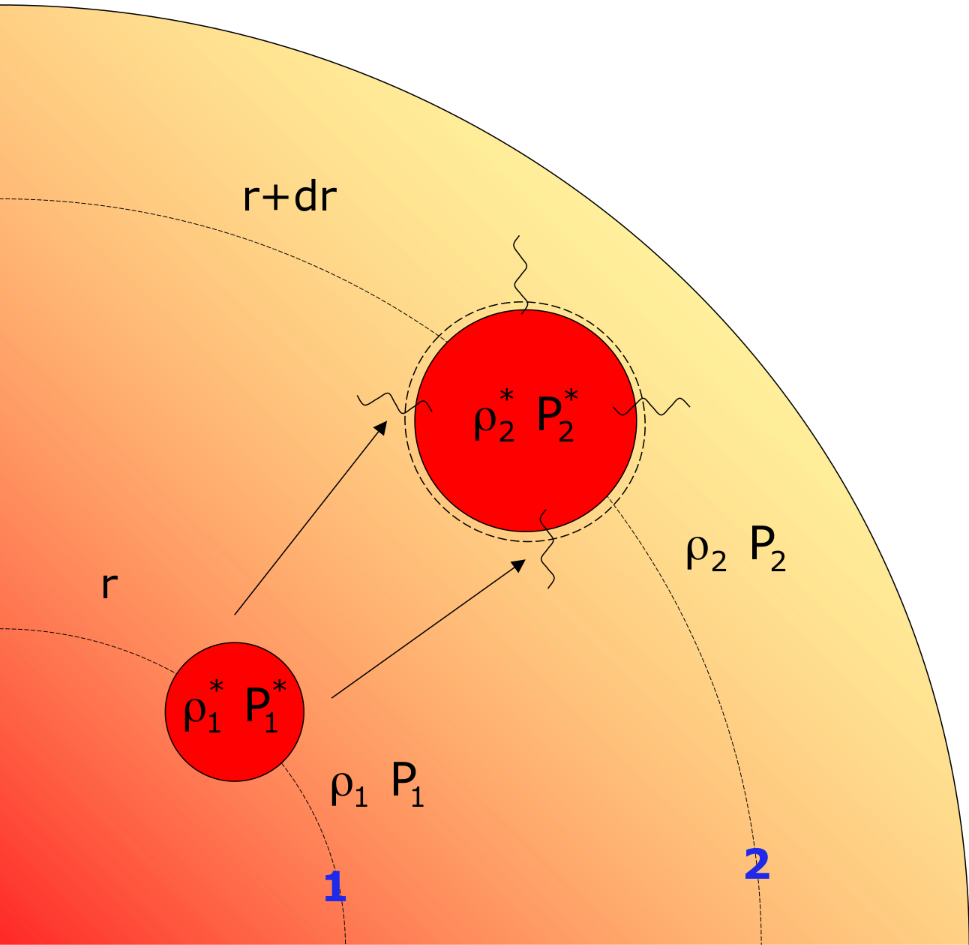
\includegraphics[width=0.3\textwidth]{immagini/criterio-schwarzscild.png}
\caption{Raffigurazione del criterio di Schwarzscild. Se la bolla si sposta dalla posizione $1$ a $2$, può avvenire la convezione solamente se ${\rho_2}^* < \rho_2$. In caso contrario siamo in presenza di equilibrio stabile e la bolla viene respinta verso la posizione iniziale.}
\label{fig:criterio-schwarzscild}
\end{figure}

Per capire il criterio~\eqref{eq:criterio-schwarzscild} consideriamo (fig.~\ref{fig:criterio-schwarzscild}) una bolla di gas in una posizione $1$ a distanza $r$ rispetto al centro, di densità ${\rho_1}^*$ e pressione interna ${P_1}^*$. Siano $\rho_1$ e $P_1$ rispettivamente la densità e la pressione dell'ambiente circostante la bolla in quella posizione. Immagino che essa si sposti in una posizione $2$ a distanza $r + \ud r$ dal centro, avendo una nuova densità ${\rho_2}^*$ e una nuova pressione interna ${P_2}^*$. Analogamente a prima, siano $\rho_2$ e $P_2$ rispettivamente la densità e la pressione dell'ambiente circostante la bolla in quella posizione. Ho convezione nella stella solo se l'equilibrio è instabile, perché in caso di equilibrio stabile la bolla tenderebbe a tornare nella posizione originaria $1$ e non sarebbe possibile lo spostamento di porzioni di gas nella stella. La condizione di equilibrio dipende dal rapporto della densità interna della bolla nel secondo caso, ${\rho_2}^*$, e la densità del gas circostante, $\rho_2$. In particolare:
\begin{subequations}
\label{eq:relazioni-densità-schwarzscild}
\begin{align}
  \text{se} \quad {\rho_2}^* &> \rho_2 \implies \text{la bolla torna nella posizione iniziale $1$.} \\
  \text{se} \quad {\rho_2}^* &< \rho_2 \implies \text{la bolla continua ad andare verso l'alto.} 
\end{align}
\end{subequations}
ed è semplice tradurre le espressioni~\eqref{eq:relazioni-densità-schwarzscild} in termini dei gradienti di temperatura, ottenendo~\eqref{eq:criterio-schwarzscild}.

\subsection{Esempio per il gas perfetto}
\begin{figure}
\centering
\subfloat[][\emph{Caso in cui avviene la convezione: modulo del gradiente radiativo maggiore del gradiente adiabatico.} \label{fig:criterio-schwarzscild-gas-perfetto1}]
{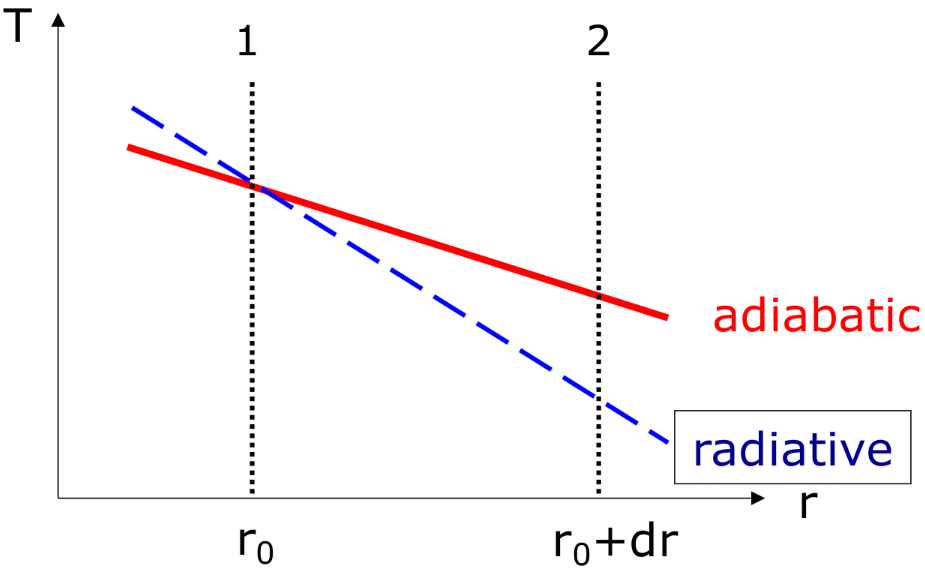
\includegraphics[width=.35\textwidth]{immagini/criterio-schwarzscild-gas-perfetto1.png}} \qquad
\subfloat[][\emph{Caso in cui non avviene la convezione: modulo del gradiente radiativo minore del gradiente adiabatico.}\label{fig:criterio-schwarzscild-gas-perfetto2}]
{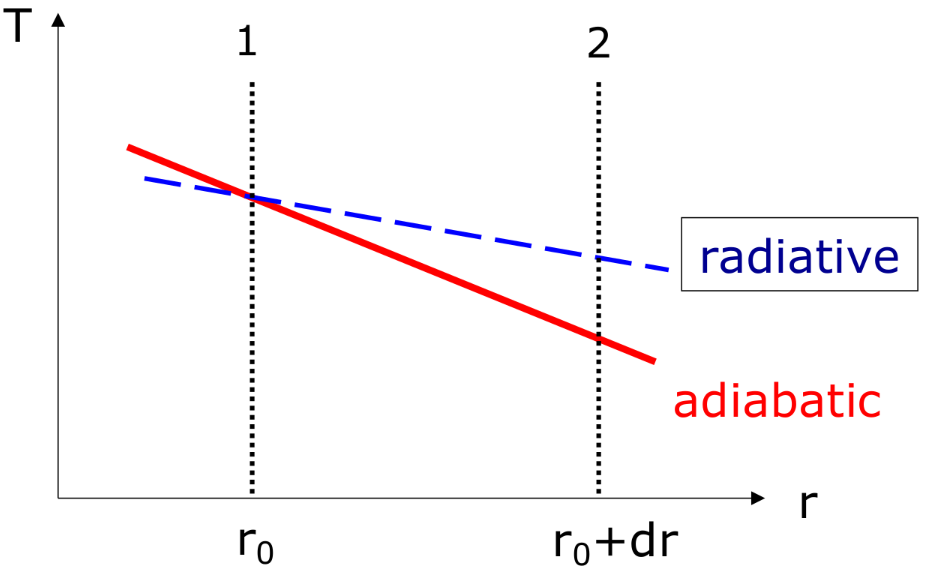
\includegraphics[width=.35\textwidth]{immagini/criterio-schwarzscild-gas-perfetto2.png}} 
\caption{Applicazione del criterio di Schwarzscild nel caso di un gas perfetto.}
\label{fig:criterio-schwarzscild-gas-perfetto}
\end{figure}

Per capire meglio le condizioni~\eqref{eq:relazioni-densità-schwarzscild} e il criterio di Schwarzscild~\eqref{eq:criterio-schwarzscild}, consideriamo il caso di un gas perfetto, in cui vale la legge~\eqref{eq:gas-ideale}. Si faccia riferimento alla figura~\ref{fig:criterio-schwarzscild-gas-perfetto}. Consideriamo un caso in cui è possibile la convezione e un caso in cui essa non è possibile

\paragraph{Convezione possibile}
Nel caso illustrato nella figura~\ref{fig:criterio-schwarzscild-gas-perfetto1} la convezione è possibile, infatti in quel caso si ha:
\[
\abs*{\dfrac{\ud T}{\ud r}}_\textup{rad} > \abs*{\dfrac{\ud T}{\ud r}}_\textup{ad}
\]
si faccia attenzione al fatto che nel criterio di Schwarzscild~\eqref{eq:criterio-schwarzscild} i gradienti sono espressi in modulo, quindi bisogna guardare la pendenza in modulo delle rette. In particolare, la bolla di gas di sposta da $r_0$ fino a $r_0 + \ud r$ e nella posizione $r_0 + \ud r$ possiede una temperatura (curva rossa -- profilo adiabatico) maggiore dell'ambiente circostante (curva blu -- profilo radiativo). Per un gas perfetto, secondo la ~\eqref{eq:gas-ideale}, a fissata pressione, a una maggiore temperatura corrisponde una densità più bassa. Quindi la bolla possiede una densità più bassa dell'ambiente circostante e tende a continuare il suo moto verso l'esterno. È dunque possibile la convezione.

\paragraph{Convezione impossibile}
Nel caso illustrato nella figura~\ref{fig:criterio-schwarzscild-gas-perfetto2} la convezione \emph{non} è possibile, infatti in quel caso si ha:
\[
\abs*{\dfrac{\ud T}{\ud r}}_\textup{rad} < \abs*{\dfrac{\ud T}{\ud r}}_\textup{ad}
\]
In particolare, la bolla di gas di sposta da $r_0$ fino a $r_0 + \ud r$ e nella posizione $r_0 + \ud r$ possiede una temperatura (curva rossa -- profilo adiabatico) minore dell'ambiente circostante (curva blu -- profilo radiativo). Per un gas perfetto, secondo la ~\eqref{eq:gas-ideale}, a fissata pressione, a una minore temperatura corrisponde una densità più alta. Quindi la bolla possiede una densità più alta dell'ambiente circostante e viene respinta verso la posizione iniziale a $r_0$.

\subsection{Gradiente di pressione e scala logaritmica}
Il criterio di Schwarzscild è spesso scritto usando il gradiente di temperatura riferito alla \emph{pressione} invece che al raggio, e in scala logaritmica. Questo perché la temperatura è intimamente connessa con la pressione.
\begin{equation}
    \dfrac{\ud T}{\ud P} \dfrac{P}{T} = \dfrac{\ud \log T}{\ud \log P} \equiv \nabla
\end{equation}
L'impiego di $\nabla$ semplifica la formulazione del criterio. Ad esempio, possiamo riscrivere l'espressione del gradiente adiabatico~\eqref{eq:gradiente-adiabatico} nella seguente maniera:
\[
\Bigl(1- \frac{1}{\gamma}\Bigr) = \dfrac{P}{T} \dfrac{\ud r}{\ud P} \dfrac{\ud T}{\ud r}\Big|_\textup{ad} = \dfrac{P}{T} \dfrac{\ud T}{\ud P}\Big|_\textup{ad}
\]
da cui:
\begin{equation}
    \nabla_\textup{ad} = \Bigl(1- \frac{1}{\gamma}\Bigr)
\end{equation}
che è semplicemente un numero. In particolare, con $\gamma = 5/3$ si ottiene $\nabla_\textup{ad} = 0.4$ ed è possibile riscrivere il criterio di Schwarzscild~\eqref{eq:criterio-schwarzscild} nella seguente materia:
\begin{equation}\label{eq:criterio-schwarzscild-nabla}
    \text{se} \quad \nabla_\textup{rad} > \nabla_\textup{ad} \implies \text{c'è convezione.}
\end{equation}
Si faccia riferimento alla figura~\ref{fig:criterio-schwarzscild-nabla} per un sunto del criterio.

\begin{figure}
\centering
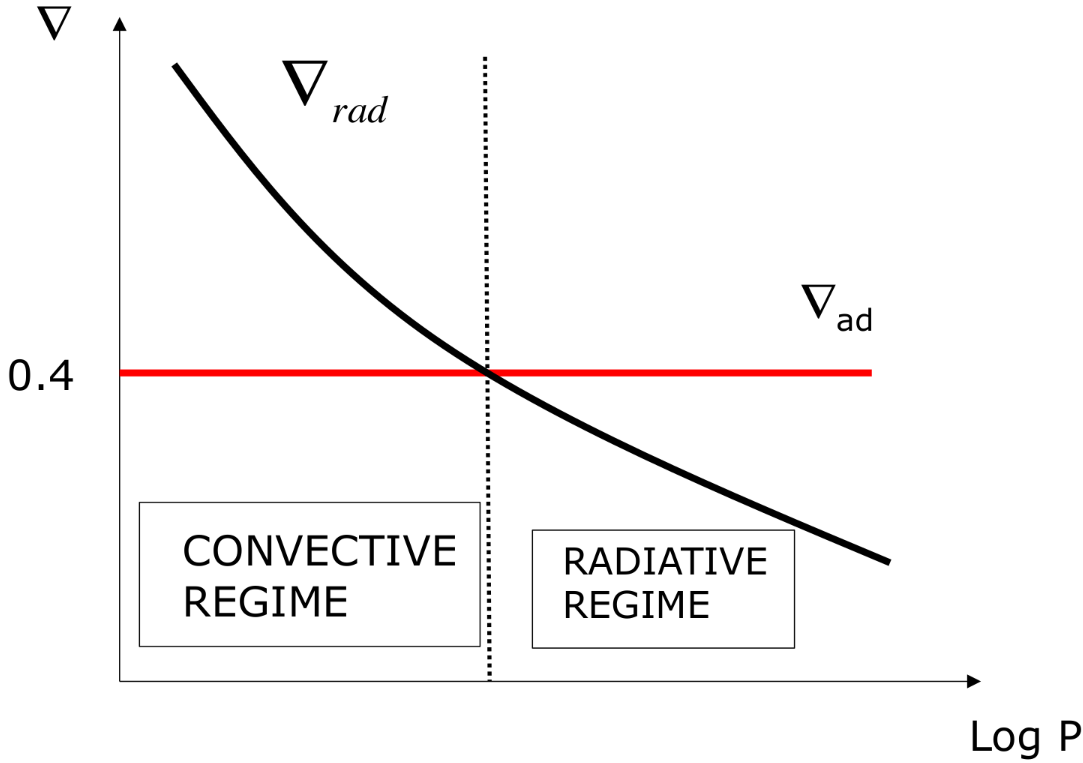
\includegraphics[width=0.4\textwidth]{immagini/criterio-schwarzscild-nabla.png}
\caption{Raffigurazione del criterio di Schwarzscild utilizzando $\nabla$.}
\label{fig:criterio-schwarzscild-nabla}
\end{figure}